\begin{frame}
	\frametitle{Analyseur syntaxique}
	\begin{itemize}
	\item Objectif double~: 
		\begin{itemize}
		\item vérifier la validité du programme écrit
		\item générer un arbre abstrait analysable par l'analyseur sémantique
		\end{itemize}
	\item Langage utilisé~: GNU Bison (Yacc)
	\end{itemize}
\end{frame}

\begin{frame}[fragile]
	\begin{rail}
		selection : IF expr statement \\ (ELSE statement) ? ;
	\end{rail}
\end{frame}

\begin{frame}[fragile]
	Code~:
	\begin{lstlisting}[language=Stibbons]
new agent {
  a = 10
  fd a + 2
}
	\end{lstlisting}
	Jetons~:
	\begin{lstlisting}[breaklines]
<NEW> <AGT> <{> <\n> 
  <ID,"a"> <=> <NUMBER,10> <\n>
  <FD> <ID,"a"> <+> <NUMBER,2> <\n>
<}>
	\end{lstlisting}
\end{frame}

\begin{frame}
L'exemple précédent génère l'arbre abstrait suivant~:
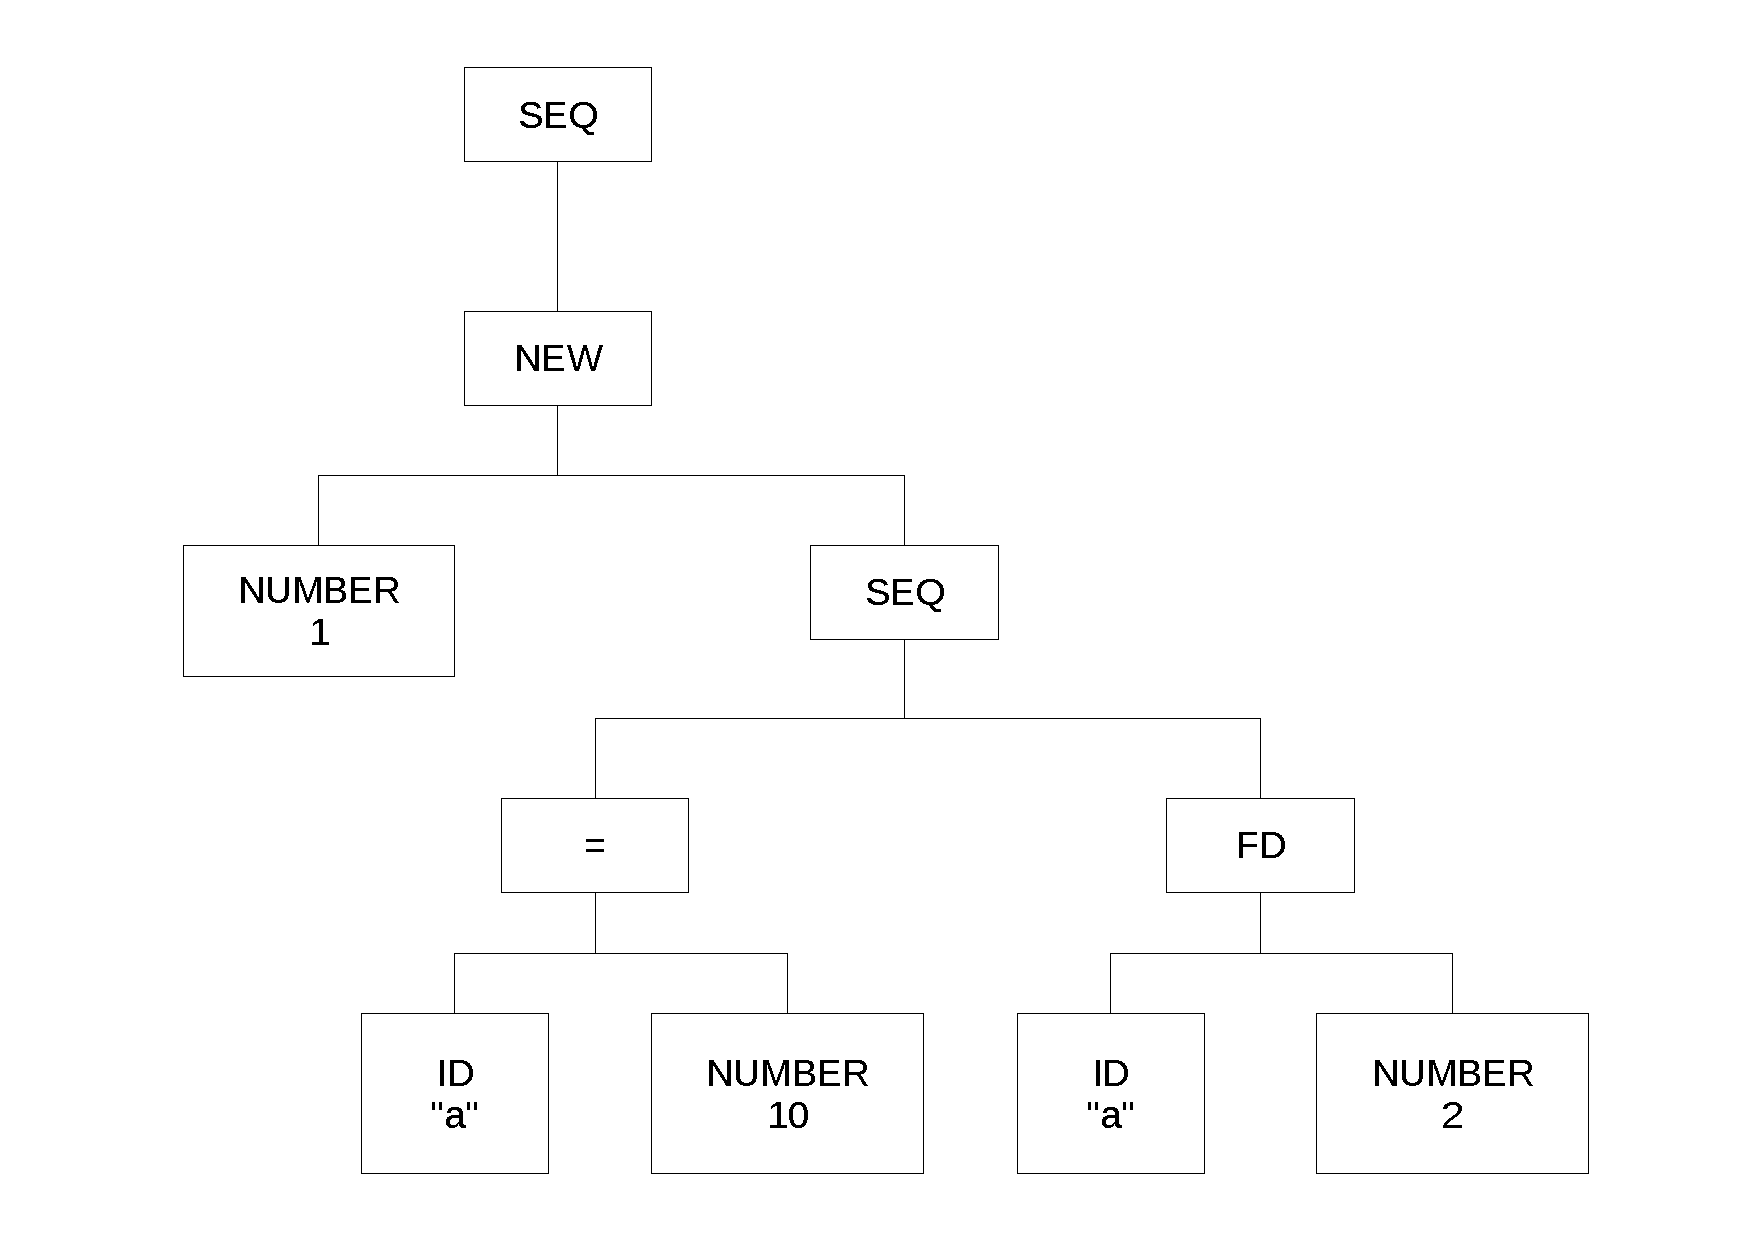
\includegraphics[scale=0.3]{doc/Presentation/img/arbre.pdf}
\end{frame}
